\subsection{NetShaper Does Not Limit Bandwidth Utilisation}
\label{subsec:netshaper-evaluation-bw}

We first evaluate if NetShaper affects the bandwidth utilisation of the underlying 10G links.
We configure NetShaper middleboxes with $k = 2$ \textit{data streams}
\footnote{\textit{iPerf3} sets up a control connection with the server for coordinating the test setup and a data connection for the test traffic.}.
We fix the output bitrate of \textit{iPerf3} and increase it until the bandwidth utilisation reported by \textit{iPerf3} is less than the set bitrate.
\textit{iPerf3} reports the bandwidth utilisation every 10 seconds.
We run this test for 180 seconds and discard the first 30 seconds reported.
As we can see in \Cref{fig:netshaper-eval-bw}, \textit{iPerf3} achieves the same bandwidth utilisation with and without NetShaper.

\begin{figure}[!htb]
    \centering
    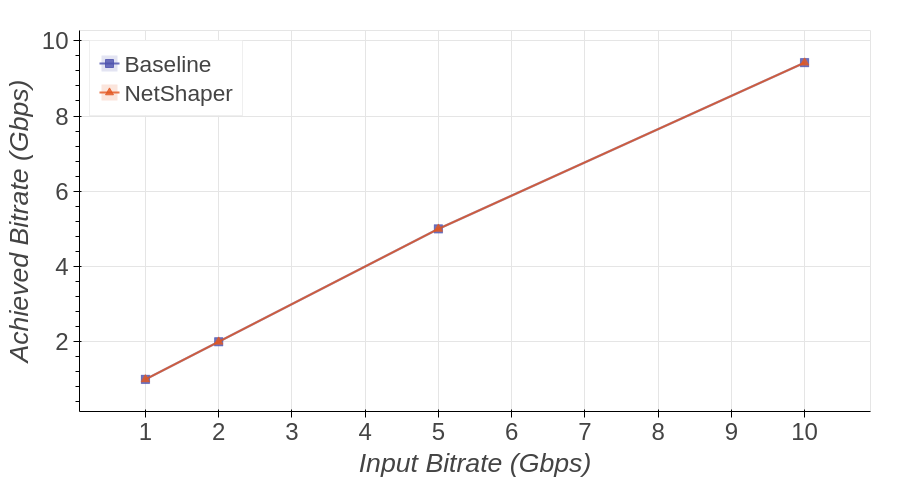
\includegraphics[width=\columnwidth]{figures/netshaper/evaluation/bw.png}
    \caption{Impact of NetShaper on Bandwidth Utilisation}
    \label{fig:netshaper-eval-bw}
\end{figure}